\documentclass{beamer}

\mode<presentation>
{
\usetheme[width=0.7in]{Hannover}
}

\usepackage[english]{babel}
\usepackage{amsthm}

\usepackage{times}
\usepackage{physics}
\usepackage{yquant}


\usepackage{subcaption}
\usepackage{tikz}
\usetikzlibrary{quantikz,fit,quotes,svg.path}
\newcommand{\h}[1]{\mintinline{haskell}{#1}}

\newcommand{\x}{\textsc{x}}
\newcommand{\cx}{\textsc{cx}}
\newcommand{\ccx}{\textsc{ccx}}
\newcommand{\cccx}{\textsc{cccx}}
\newcommand{\qket}[1]{\ket{\tilde{#1}}}
\newcommand{\preim}[2]{\{\cdot\stackrel{#1}{\longleftarrow}{#2}\}}
\newcommand{\finset}[1]{[\mathbf{#1}]}
\newcommand{\red}[1]{{\color{red}{#1}}}
\newcommand{\Bool}{\ensuremath{\mathbb{B}}}

\usepackage{multirow}
\usepackage{totpages}
\usepackage{hyperref}
\usepackage{booktabs}

\hypersetup{
  urlcolor=blue,
  linkcolor=blue,
  colorlinks=true
}

\newtheorem{defn}{Definition}
\newtheorem{prob}{Problem}

\usepackage{listings}
\lstset{columns=flexible,
        language=haskell}
%\usepackage{tikz}
%\usetikzlibrary{positioning}

\newcommand{\blt}{- } %used for bullets in a list

\newcounter{datadefnum} %Datadefinition Number
\newcommand{\ddthedatadefnum}{DD\thedatadefnum}
\newcommand{\ddref}[1]{DD\ref{#1}}

\newcommand{\colAwidth}{0.1\textwidth}
\newcommand{\colBwidth}{0.8\textwidth}

\renewcommand{\arraystretch}{1.1} %so that tables with equations do not look 
%crowded

\pgfdeclareimage[height=0.7cm]{logo}{McMasterLogo}
\title[\pgfuseimage{logo}] % (optional, use only with long paper titles)
{Partial Evaluation of (Quantum) Circuits}

\author[]{\underline{Jacques Carette}, Amr Sabry, Gerardo Ortiz}

\date[Aug 18, 2022] % (optional, should be abbreviation of conference name)
{WG 2.11, Odense, Denmark}

\pgfdeclareimage[height=0.5cm]{Mac-logo}{McMasterLogo}
\logo{\pgfuseimage{Mac-logo}}

% Delete this, if you do not want the table of contents to pop up at
% the beginning of each subsection:
% \AtBeginSubsection[]
% {
%   \begin{frame}<beamer>
%     \frametitle{Outline}
%     \tableofcontents[currentsection,currentsubsection]
%   \end{frame}
% }

% If you wish to uncover everything in a step-wise fashion, uncomment
% the following command: 

%\beamerdefaultoverlayspecification{<+->}

\beamertemplatenavigationsymbolsempty 

\usepackage{color}

%\newcommand{\authornote}[3]{\textcolor{#1}{[#3 ---#2]}}
%\newcommand{\jc}[1]{\authornote{purple}{JC}{#1}}

%% Useful abbreviations

\newcommand{\pub}[1]{\textcolor{purple}{#1}}
\begin{document}

%%%%%%%%%%%%%%%%%%%%%%%%%%%%%%%%%%%%%%
\hoffset=-.4in %removing side bar for these frames
\begin{frame}[plain]

\titlepage

\end{frame}
\hoffset=0in %restore

%%%%%%%%%%%%%%%%%%%%%%%%%%%%%%%%%%%%%%

\section[Introduction]{Introduction}

%%%%%%%%%%%%%%%%%%%%%%%%%%%%%%%%%%%%%%

\begin{frame}

\frametitle{Quantum Circuit}

\begin{figure}[b]
  \centering
\begin{subfigure}[b]{.25\textwidth}
    \centering
    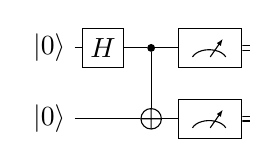
\begin{tikzpicture}[scale=1.0]
   \begin{yquant*}[register/minimum height=0.8cm]
   qubit {$\ket0$} x;
   qubit {$\ket0$} y;
   box {$H$} x;
   cnot y | x;
   measure x;
   measure y;
  \end{yquant*}
\end{tikzpicture}
\caption{\label{fig:bell}Bell circuit}
\end{subfigure}
\qquad
\begin{subfigure}[b]{.25\textwidth}
    \centering
    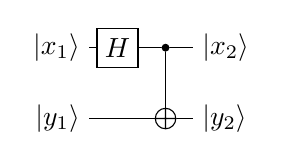
\begin{tikzpicture}[scale=1.0]
   \begin{yquant*}[register/minimum height=0.8cm]
   qubit {$\ket{x_1}$} x;
   qubit {$\ket{y_1}$} y;
   box {$H$} x;
   cnot y | x;
   output {$\ket{x_2}$} x;
   output {$\ket{y_2}$} y;
  \end{yquant*}
\end{tikzpicture}
\caption{\label{fig:bellqcore}Quantum core}
\end{subfigure}
\qquad
\begin{subfigure}[b]{.25\textwidth}
    \centering
    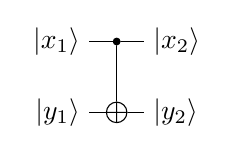
\begin{tikzpicture}[scale=1.0]
   \begin{yquant*}[register/minimum height=0.8cm]
   qubit {$\ket{x_1}$} x;
   qubit {$\ket{y_1}$} y;
   cnot y | x;
   output {$\ket{x_2}$} x;
   output {$\ket{y_2}$} y;
  \end{yquant*}
\end{tikzpicture}
\caption{\label{fig:bellccore}Classical core}
\end{subfigure}
%\caption{\label{fig:bellall}A conventional quantum circuit with
%  initial conditions and measurement (a); its quantum core without
%  measurement and with unspecified initial and final conditions (b); and
%  its classical core without explicit quantum superpositions (c).}
\end{figure}

Legend:
  $$ \ket{0} = \text{false} = 0 $$
  $$ \ket{1} = \text{true} = 1 $$
\end{frame}

%%%%%%%%%%%%%%%%%%%%%%%%%%%%%%%%%%%%%%

\section[Examples]{Examples}

%%%%%%%%%%%%%%%%%%%%%%%%%%%%%%%%%%%%%%

\begin{frame}

\frametitle{Examples part I}

\begin{figure}[b]
    \centering
    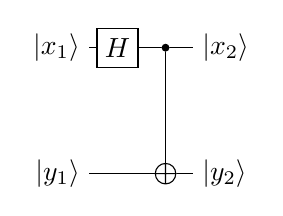
\begin{tikzpicture}[scale=1.0]
   \begin{yquant*}[register/minimum height=1.5cm]
   qubit {$\ket{x_1}$} x;
   qubit {$\ket{y_1}$} y;
   box {$H$} x;
   cnot y | x;
   output {$\ket{x_2}$} x;
   output {$\ket{y_2}$} y;
  \end{yquant*}
\end{tikzpicture}
\caption{\label{fig:bellqcore2}Quantum core}
\end{figure}

\end{frame}

%%%%%%%%%%%%%%%%%%%%%%%%%%%%%%%%%%%%%%

\begin{frame}

\frametitle{Examples part II}

\begin{figure}[b]
    \centering
  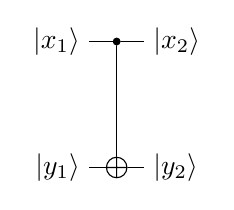
\begin{tikzpicture}[scale=1.0]
   \begin{yquant*}[register/minimum height=1.5cm]
   qubit {$\ket{x_1}$} x;
   qubit {$\ket{y_1}$} y;
   cnot y | x;
   output {$\ket{x_2}$} x;
   output {$\ket{y_2}$} y;
   \end{yquant*}
  \end{tikzpicture}
\caption{\label{fig:bellccore2}Classical core}
\end{figure}

\end{frame}

%%%%%%%%%%%%%%%%%%%%%%%%%%%%%%%%%%%%%%

\begin{frame}

\frametitle{Real Examples}

\begin{enumerate}
  \item Deutsch
  \item Deutsch-Jozsa
  \item Bernstein-Varizani
  \item Simon
  \item Grover
  \item Shor
\end{enumerate}

\pause

\vspace*{1cm}
\red{caveat: Black-Box vs White Box}

\end{frame}

%%%%%%%%%%%%%%%%%%%%%%%%%%%%%%%%%%%%%%

\begin{frame}

\frametitle{Deutsch}

  \begin{prob}
Given $f : \Bool\rightarrow\Bool$, decide if $f$ is 
\emph{constant} or \emph{balanced}.
  \end{prob}

\pause

\begin{defn}
  A boolean function is \textbf{balanced} if it outputs the same number of
  0/1 outputs.
\end{defn}

\pause

\vspace*{1cm}
$\ket{x}\ket{y} \rightarrow\ket{x}\ket{f(x)\oplus y}$
\end{frame}


%%%%%%%%%%%%%%%%%%%%%%%%%%%%%%%%%%%%%%

\begin{frame}

\frametitle{Deutsch-Josza}

  \begin{prob}Given $f : \Bool^n\rightarrow\Bool$, where $f$ is known to be
\emph{constant} or \emph{balanced}, decide which one it is.
  \end{prob}

\pause

Sample outputs:
\begin{itemize}
\item $0 = 0$
\item $x_0 = 0$,
\item $x_0 \oplus x_1 \oplus x_2 \oplus x_3 \oplus
    x_4 \oplus x_5 = 0$, and
\item $1 \oplus x_3x_5 \oplus x_2x_4 \oplus x_1x_5
\oplus x_0x_3 \oplus x_0x_2 \oplus x_3x_4x_5 \oplus x_2x_3x_5 \oplus
x_1x_3x_5 \oplus x_0x_3x_5 \oplus x_0x_1x_4 \oplus x_0x_1x_2 \oplus
x_2x_3x_4x_5 \oplus x_1x_3x_4x_5 \oplus x_1x_2x_4x_5 \oplus
x_1x_2x_3x_5 \oplus x_0x_3x_4x_5 \oplus x_0x_2x_4x_5 \oplus
x_0x_2x_3x_5 \oplus x_0x_1x_4x_5 \oplus x_0x_1x_3x_5 \oplus
x_0x_1x_3x_4 \oplus x_0x_1x_2x_4 \oplus x_0x_1x_2x_4x_5 \oplus
x_0x_1x_2x_3x_5 \oplus x_0x_1x_2x_3x_4 = 0$.
\end{itemize}

  But how to \emph{decide}? Easy: if it mentions a variable, it's balanced.
\end{frame}

%%%%%%%%%%%%%%%%%%%%%%%%%%%%%%%%%%%%%%

\begin{frame}

\frametitle{Bernstein-Varizani, Simon}

Bernstein-Varizani
\begin{prob}
    Given $f : \Bool^n\rightarrow\Bool$, where $f$ is known to be
of the shape $\sum_i s_i x_i \mod 2$ for some $s\in\Bool^n$ and $s_i$ is its
bit decomposition. Find $s$.
\end{prob}

\pause

Simon
\begin{prob}
    Given $f : \Bool^n\rightarrow\Bool$, where it is known that
    there exist $a$ such that $\forall x. f(x) = f(x + a)$. Find $a$.
\end{prob}

\end{frame}

%%%%%%%%%%%%%%%%%%%%%%%%%%%%%%%%%%%%%%

\begin{frame}

  \frametitle{Grover}

\begin{prob}
    Given $f : \Bool^n\rightarrow\Bool$ where there exists a unique $x$
    such that $f(x)=1$. Find $x$.
\end{prob}

\pause

$n=4$, $w$ in the range $\{0..15\}$
  {\tiny
\begin{tabular}{ll}
$u=0$ & 
  $\red{1} \oplus x_3 \oplus x_2 \oplus x_1 \oplus x_0 \oplus x_2x_3 \oplus x_1x_3 \oplus x_1x_2 \oplus x_0x_3 \oplus x_0x_2 \oplus x_0x_1 \oplus x_1x_2x_3 \oplus x_0x_2x_3$ \\
   &\quad $\oplus ~x_0x_1x_3 \oplus x_0x_1x_2 \oplus x_0x_1x_2x_3$ \\
$u=1$ & 
  $\red{x_0} \oplus x_0x_3 \oplus x_0x_2 \oplus x_0x_1 \oplus x_0x_2x_3 \oplus x_0x_1x_3 \oplus x_0x_1x_2 \oplus x_0x_1x_2x_3$ \\
$u=2$ &
  $\red{x_1} \oplus x_1x_3 \oplus x_1x_2 \oplus x_0x_1 \oplus x_1x_2x_3 \oplus x_0x_1x_3 \oplus x_0x_1x_2 \oplus x_0x_1x_2x_3$ \\
$u=3$ &
  $\red{x_0x_1} \oplus x_0x_1x_3 \oplus x_0x_1x_2 \oplus x_0x_1x_2x_3$ \\
$u=4$ &
  $\red{x_2} \oplus x_2x_3 \oplus x_1x_2 \oplus x_0x_2 \oplus x_1x_2x_3 \oplus x_0x_2x_3 \oplus x_0x_1x_2 \oplus x_0x_1x_2x_3$ \\
$u=5$ &
  $\red{x_0x_2} \oplus x_0x_2x_3 \oplus x_0x_1x_2 \oplus x_0x_1x_2x_3$ \\
$u=6$ &
  $\red{x_1x_2} \oplus x_1x_2x_3 \oplus x_0x_1x_2 \oplus x_0x_1x_2x_3$ \\
$u=7$ &
  $\red{x_0x_1x_2} \oplus x_0x_1x_2x_3$ \\
$u=8$ &
  $\red{x_3} \oplus x_2x_3 \oplus x_1x_3 \oplus x_0x_3 \oplus x_1x_2x_3 \oplus x_0x_2x_3 \oplus x_0x_1x_3 \oplus x_0x_1x_2x_3$ \\
$u=9$ &
  $\red{x_0x_3} \oplus x_0x_2x_3 \oplus x_0x_1x_3 \oplus x_0x_1x_2x_3$ \\
$u=10$ &
  $\red{x_1x_3} \oplus x_1x_2x_3 \oplus x_0x_1x_3 \oplus x_0x_1x_2x_3$ \\
$u=11$ &
  $\red{x_0x_1x_3} \oplus x_0x_1x_2x_3$ \\
$u=12$ &
  $\red{x_2x_3} \oplus x_1x_2x_3 \oplus x_0x_2x_3 \oplus x_0x_1x_2x_3$ \\
$u=13$ &
  $\red{x_0x_2x_3} \oplus x_0x_1x_2x_3$ \\
$u=14$ &
  $\red{x_1x_2x_3} \oplus x_0x_1x_2x_3$ \\
$u=15$ &
  $\red{x_0x_1x_2x_3}$
\end{tabular}
  }

\end{frame}

%%%%%%%%%%%%%%%%%%%%%%%%%%%%%%%%%%%%%%

\begin{frame}

  \frametitle{Shor}

\begin{prob}
  Factor a given $N$. Do this by using $f(x) = a^x \mod N$ for suitable $a$ and
  $f : \Bool^Q \rightarrow \Bool^Q$ with $Q = \lceil \log_2 \left(N^2\right) \rceil$.
\end{prob}

  {\tiny
\[\begin{array}{l@{\quad}lllll}
  \hspace*{-8mm}\textrm{Base} & \multicolumn{4}{c}{\textrm{Equations}} & \textrm{Solution} \\[2ex]
  \hspace*{-8mm} a=11 & x_0 = 0 &&&& \red{x_0 = 0} \\
  \hspace*{-8mm} a=4,14 & 1 \oplus x_0 = 1 & x_0 = 0 && & \red{x_0 = 0} \\
  \hspace*{-8mm} a=7,13 & 1 \oplus x_1 \oplus x_0x_1 = 1 & x_0x_1 = 0 & x_0 \oplus x_1 \oplus x_0x_1 = 0 &  x_0 \oplus x_0x_1 = 0 & \red{x_0=x_1=0} \\
  \hspace*{-8mm} a=2,8 & 1 \oplus x_0 \oplus x_1 \oplus x_0x_1 = 1 & x_0x_1 = 0 & x_1 \oplus x_0x_1 = 0 & x_0 \oplus x_0x_1 = 0  & \red{x_0=x_1=0}
\end{array}\]
  }

  Auto-generated circuits: 56,538 generalized Toffoli gates. 

  \pause
  \vspace*{4mm}
  For 3*65537=196611 (4,328,778 gates),
   16 small equations that refer to just the four variables $x_0$, $x_1$, $x_2$, and $x_3$
constraining them to be all 0, i.e.,
asserting that the period is 16.
\end{frame}

\end{document}
